\documentclass[a4paper,12pt]{article} % Article document, A4 paper, 10pt font size
\usepackage[utf8]{inputenc} % UTF-8 input encoding
\usepackage[T1]{fontenc}    % T1 (vector) fonts
\usepackage{lmodern}        % Latin Modern (vector) font
\usepackage{microtype}      % Typographic improvements

\usepackage[english]{babel} % English typographic and hyphenation patterns

\usepackage{amsmath}        % American Mathematical Society commands
\usepackage{amsfonts}       % AMS fonts
\usepackage{bbold} 
\usepackage{amssymb}        % AMS symbols
\usepackage{amsthm}         % AMS theorem environments
\usepackage{mathtools}
\usepackage{tabularx}
\usepackage{graphicx}       % Graphics
\usepackage{wrapfig}
\usepackage{float}

\usepackage[utf8]{inputenc}
\usepackage[T1]{fontenc}
\usepackage{babel}
\usepackage{amsmath,amsfonts,amssymb}
\usepackage{subcaption}	

\usepackage[dvipsnames]{xcolor} 
\usepackage{listings}
\usepackage{xcolor}
\usepackage{caption}
\DeclareCaptionFont{white}{\color{white}}
\DeclareCaptionFormat{listing}{\colorbox{gray}{\parbox{\textwidth}{#1#2#3}}}
\DeclareMathOperator{\ind}{\perp \!\!\! \perp}
\captionsetup[lstlisting]{format=listing,labelfont=white,textfont=white}

% set the default code style
\lstset{
belowcaptionskip=1\baselineskip,
  breaklines=true,
  numbers=left,
  numberstyle=\small,
  frame=single,
  xleftmargin=\parindent,
  language=Python,
  showstringspaces=false,
  basicstyle=\footnotesize\ttfamily,
  keywordstyle=\bf\color{green!40!black},
  commentstyle=\itshape\color{Aquamarine},
  identifierstyle=\color{blue},
  stringstyle=\color{red},
  }

% Theorem environments
\newtheorem{theorem}{Theorem}
\newtheorem{lemma}{Lemma}
\newtheorem{definition}{Definition}
\newtheorem{notation}{Notation}
\newtheorem{Demonstration}{Demonstration}
\newtheorem{corollary}{Corollary}
\newtheorem{proposition}{Proposition}

% Margins
\usepackage{geometry}
\geometry{
 a4paper,
total={170mm,257mm},
 left=25mm,
 right=25mm,
 top=20mm,
}
\newlength{\drop}

\begin{document}

\begin{center}
    \drop=0.1\textheight
    \centering
    \vspace*{\baselineskip}
    \rule{\textwidth}{1.6pt}\vspace*{-\baselineskip}\vspace*{2pt}
    \rule{\textwidth}{0.4pt}\\[\baselineskip]
    {\huge {\textbf{HOMEWORK 2 : MAP estimation on NMF}}
    \rule{\textwidth}{0.4pt}\vspace*{-\baselineskip}\vspace{3.2pt}
    \rule{\textwidth}{1.6pt}\\[\baselineskip]
    \vspace*{\baselineskip}
    \scshape
    Introduction to Probabilistic Graphical Models   \par
    \vspace*{2\baselineskip}\
    Authored by \\[\baselineskip]
    {\Large MARION KARAKOUZIAN \\ \& \\
    YASSINE BENAZZOU \\ \& \\
    MEHDI ABBANA BENNANI \par}\ \\
    \vspace*{\baselineskip}\
    Professor \\
    {\Large Umut Simsekli  \par}\ \\
    {\itshape Ecole Polytechnique \par}
    \vfill
    {\scshape 2017} \        \par
}  \end{center}
  
\newpage

\section{Exercise 1}
We have that $\hat{V}=WH$, $w_{fk} \sim G(\alpha_w,\beta_w)$, $h_{kn} \sim G(\alpha_h,\beta_h)$ and $v_{fn}|w_{f,:},h_{:,n} \sim \mathcal{P}(\langle w_{f,:},h_{:,n}\rangle)$. 

\begin{align*}
\langle W^*,H^*\rangle \: &= \underset{(W,H)}{\mathrm{argmax}} \log (P(W,H|V))\\
&= \underset{(W,H)}{\mathrm{argmax}} \log (\frac{P(V|W,H)\times P(W,H)}{P(V)}) \\
&= \underset{(W,H)}{\mathrm{argmax}} \log (P(V|W,H))+\log (P(W,H))\\
&= \underset{(W,H)}{\mathrm{argmax}} \sum\limits_{fn}\left( V_{fn}\times \log(\hat{V}_{fn}) - \hat{V}_{fn}\right) + \log (P(W,H))
\end{align*}

\begin{align*}
\log(P(W,H)) \: &= \sum\limits_{fk}\log P(w_{fk})+\sum\limits_{kn}\log P(h_{kn}) \\
&= \underset{(W,H)}{\mathrm{argmax}}\left(\sum\limits_{fn}V_{fn}\times \log(\hat{V}_{fn}) - \hat{V}_{fn}\right)+\sum\limits_{fk} \log \frac{w_{fk}^{\alpha_w-1}\times \exp(-w_{fk} \times \beta_w) \times \beta_{w}^{\alpha_w}} {\Gamma(\alpha_w)} \\
&+ \sum\limits_{kn} \log \frac{h_{kn}^{\alpha_h-1}\times \exp(-h_{kn} \times \beta_h) \times \beta_{h}^{\alpha_h}} {\Gamma(\alpha_h)} \\
&= \underset{(W,H)}{\mathrm{argmax}}[\sum\limits_{fn}(V_{fn}\times \log(\hat{V}_{fn}) - \hat{V}_{fn})+\sum\limits_{fk}((\alpha_w-1)\times \log w_{fk}-w_{fk}\times \beta_w) \\
&+ \sum\limits_{kn} ((\alpha_h-1)\log h_{kn} - \beta_h\times h_{kn})]
\end{align*}

$S_{fnk}|w_{fk},h_{kn}\sim \mathcal{P}(w_{fk},h_{kn})$

$V_{fn}|S_{fnk}\sim \delta(V_{fn}-\sum\limits_{k}S_{fnk})$\vspace{1\baselineskip}

We can apply the EM algorith, that is composed by two steps :
\begin{itemize}
\item \underline{E-step :} We have to compute \begin{align*} \mathcal{L}_t(W,H) \: &= \mathbb{E}[\log(P(V,S,W,H))]_{P(S|V,H_t,W_t)}\\
&= \mathbb{E}_{S|V,H_t,W_t}[\log P(S,V|W,H)\times P(W,H)]\times P(S|V,H_t,W_t)
\end{align*}
\item \underline{M-step :} $W_{t+1},H_{t+1}=\underset{(W,H)}{\mathrm{argmax}}\mathcal{L}_t(W,H)$\\
\end{itemize}

$\Rightarrow$ Application of the algorithm :
\begin{enumerate}
\item \underline{E-step :}
\begin{align*}
\log P(V,S|W,H) \: &= \log [P(V|S,W,H)\times P(S|W,H)]\\
&= \sum\limits_{fn} log(\delta(V_{fn}-\sum\limits_{k}S_{fnk})) + \log P(S|W,H)\\
&= \sum\limits_{fnk}\left(S_{fnk}\times \log(w_{fk}\times h_{kn})-w_{fk}\times h_{kn}-\log\Gamma(S_{fnk})\right)\\
&+ \sum\limits_{fn}\log\left(\delta(V_{fn}-\sum\limits_{k}S_{fnk})\right)
\end{align*}
\begin{align*}
\log P(W,H) = \: &\sum\limits_{fk} (\alpha_w-1)\times\log w_{fk} - w_{fk}\times\beta_w \\
&+ \sum\limits_{kn} \: (\alpha_h-1)\times\log h_{kn} - h_{kn}\times\beta_h \\
&+ ... (constant)
\end{align*}

According to the course, we have 
$\log P(S|V_t,W_t,H_t)=\log \prod\limits_{fn}M(S_{fn:},V_{fn},[\Pi_1,_,\Pi_k]^{(t)})$
with $\Pi_k^{(t)}=\frac{w_{fk}^{(t)}\times h_{kn}^{(t)}}{\hat{v}_{fn}^{(t)}}$, so we obtain
\begin{align*}
\mathcal{L}_t(W,H) = \: &\sum\limits_{fnk} \mathbb{E}[S_{fnk}]\times\log(w_{fk}\times h_{kn})-w_{fk}\times h_{kn}\\
&+ \sum\limits_{fk}(\alpha_w-1)\times\log w_{fk}-w_{fk}\times\beta_w + \sum\limits_{kn}\log h_{kn}-h_{kn}\times\beta_h\\
&+ constant
\end{align*}
\item \underline{M-step :} To compute the $\mathrm{argmax}$ of $\mathcal{L}_t$, we use the derivative :\\
\begin{align*}
\frac{\partial\mathcal{L}_t}{\partial w_{fk}}=\sum\limits_{n}\left(\frac{\mathbb{E}[S_{fnk}]}{w_{fk}}-h_{kn}^{(t)}\right)+\frac{\alpha_w-1}{w_{fk}}-\beta_w=0
\end{align*}
Then, we obtain
\begin{align*}
w_{fk}^{(t+1)} \: &= \frac{\sum\limits_{n}\mathbb{E}[S_{fnk}]+\alpha_w-1}{\beta_w+\sum\limits_{n}h_{kn}^{(t)}}\\
&= \frac{\sum\limits_{n}\left(v_{fn}\times\frac{w_{fk}^{(t)}\times h_{kn}^{(t)}}{\hat{v}_{fn}^{(t)}}\right)+\alpha_w-1}{\beta_w+\sum\limits_{n}h_{kn}^{(t)}}\\
&= \frac{w_{fk}^{(t)}\times\sum\limits_{n}\frac{v_{fn}}{\hat{v}_{fn}^{(t)}}\times h_{kn}^{(t)}+\alpha_w-1}{\beta_w+\sum\limits_{n}h_{kn}^{(t)}}
\end{align*}
Likewise for h,
$h_{kn}^{(t+1)}=\frac{h_{kn}^{(t)}\times\sum\limits_{f}\frac{v_{fn}}{\hat{v}_{fn}^{(t)}}\times w_{fk}^{(t+1)}+\alpha_h-1}{\beta_h+\sum\limits_{f}w_{fk}^{(t+1)}}$
\end{enumerate}
Finally, we have $\hat{V}=WH$, so,
\begin{align*}W\: &\leftarrow\frac{W\cdot[(V/\hat{V})H^T]+(Q_w-1)O_{FK}}{O_{FN}H^T+\beta_wO_{FK}}\\
H\: &\leftarrow\frac{H\cdot[W^T(V/\hat{V})]+(Q_w-1)O_{KN}}{W^TO_{FN}+\beta_wO_{KN}}
\end{align*}
with $\cdot$ the element-wise matrix multiplication and $/$ the element-wise division.  \\
where $O_{KN}=\left( 
\begin{array}{ccc} 
1&\cdots&1\\
\vdots&\ddots&\vdots\\
1& \cdots &1 
\end{array}
\right)$
with K lines and N columns.

\section{Exercise 2}
\paragraph{Question 1}
Please refer to the "EM\_algorithm.m" matlab code. \\

\paragraph{Question 2}

We can interpret the $W$ matrix as the projection of the faces of the $V$ matrix on a K dimensional space. Therefore every column of $W$ is a 'feature' or 'base' face. Then the $V$ matrix corresponds to the weightenings between the K faces to obtain the original faces.

The following figures show the $\Gamma$ distibution for different values of $\alpha$ and $\beta = 1$.

Therefore, we interpret the $\beta_W$ parameter as a sparsity parameter. By putting a strong prior in some region, we can tune the sparcity of the image. For the $\alpha_W$ parameter, we interpret it as the strenght of the sparsity (?)

\begin{figure}[H]
	\begin{subfigure}{.4\textwidth}
		\centering
		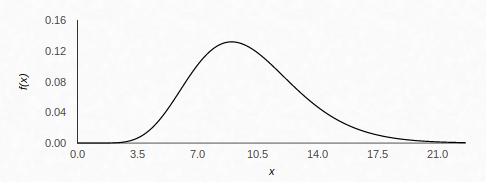
\includegraphics[width=.8\linewidth]{Gamma/Gamma_alp1_bet01.png}
		\caption{$\alpha = 1 $, $\beta = 0.1 $}
	\end{subfigure}%
	\begin{subfigure}{.4\textwidth}
		\centering
		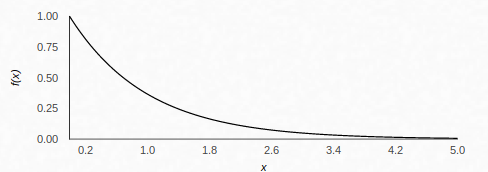
\includegraphics[width=.8\linewidth]{Gamma/Gamma_alp1_bet1.png}
		\caption{$\alpha = 1 $, $\beta = 1 $}
	\end{subfigure}%
	
	
%	\begin{subfigure}{.4\textwidth}
%		\centering
%		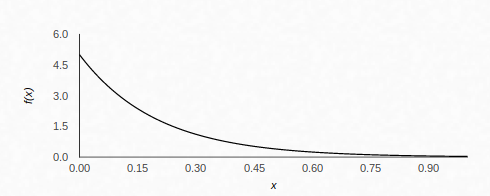
\includegraphics[width=.8\linewidth]{Gamma/Gamma_alp1_bet5.png}
%		\caption{$\alpha = 1 $, $\beta = 5 $}
%	\end{subfigure}%
	\begin{subfigure}{.4\textwidth}
		\centering
		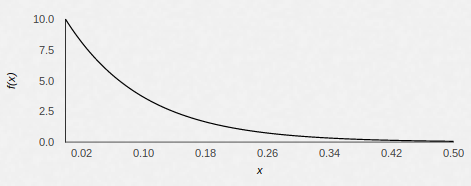
\includegraphics[width=.8\linewidth]{Gamma/Gamma_alp1_bet10.png}
		\caption{$\alpha = 1 $, $\beta = 10 $}
	\end{subfigure}%
	
	
	\begin{subfigure}{.4\textwidth}
		\centering
		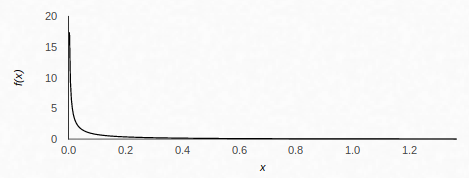
\includegraphics[width=.8\linewidth]{Gamma/Gamma_alp01_bet1.png}
		\caption{$\alpha = 0.1 $, $\beta = 1 $}
	\end{subfigure}%
	\begin{subfigure}{.4\textwidth}
		\centering
		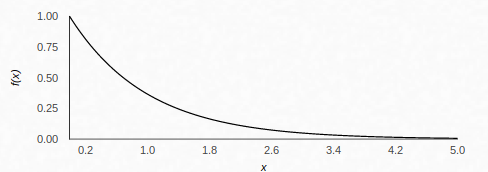
\includegraphics[width=.8\linewidth]{Gamma/Gamma_alp1_bet1.png}
		\caption{$\alpha = 1 $, $\beta = 1 $}
	\end{subfigure}%
	
		\begin{subfigure}{.4\textwidth}
		\centering
		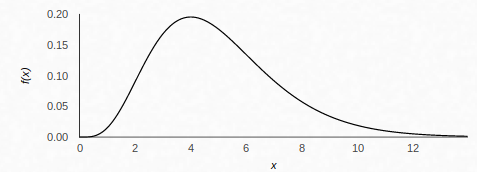
\includegraphics[width=.8\linewidth]{Gamma/Gamma_alp5_bet1.png}
		\caption{$\alpha = 5 $, $\beta = 1 $}
	\end{subfigure}%
	\begin{subfigure}{.4\textwidth}
		\centering
		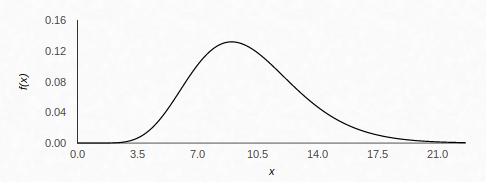
\includegraphics[width=.8\linewidth]{Gamma/Gamma_alp10_bet1.png}
		\caption{$\alpha = 10 $, $\beta = 1 $}
	\end{subfigure}%
	\caption{Gamma distribution for different values of $\alpha$ and $\beta$}
	\label{fig:Gammas}
\end{figure}   

The following figures shows the most relevant values of $\alpha$, for $\beta_w = 1$ and $\beta_h = 1$

In the first figure, we see that increasing $\alpha_W$ decreases the sparcity of the $W$ representation.

In the second figure, we see that increasing $\alpha_H$ increases the sparsity of the solution. (The weights get bigger the bigger $\alpha_H$ I expected the opposite)

\begin{figure}[H]

	\begin{subfigure}{.4\textwidth}
		\centering
		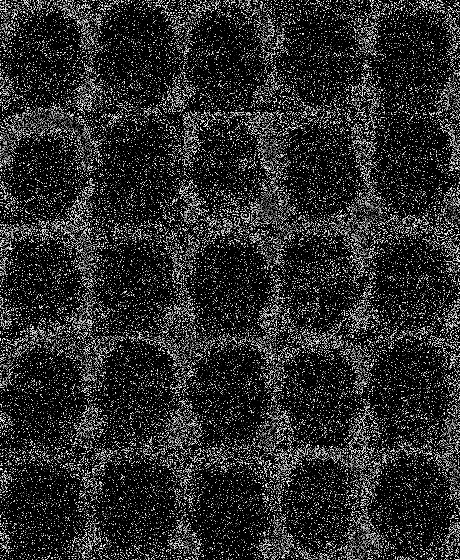
\includegraphics[width=.8\linewidth]{{betas=1/W_alph_0.1_alpw_0.1_beth_1_betw_1}.png}
		\caption{$\alpha_W = 0.1 $, $\alpha_H = 0.1 $}
	\end{subfigure}%
	\begin{subfigure}{.4\textwidth}
		\centering
		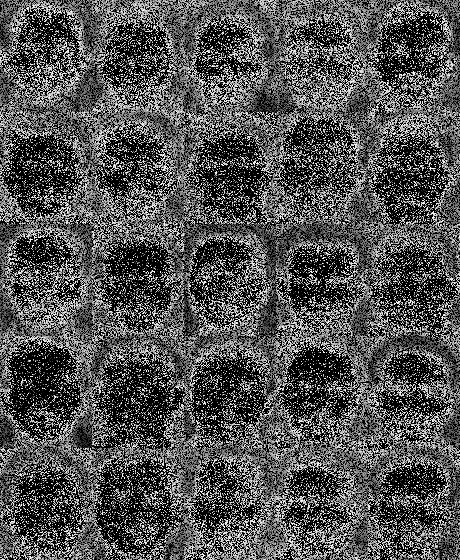
\includegraphics[width=.8\linewidth]{{betas=1/W_alph_0.1_alpw_0.2_beth_1_betw_1}.png}
		\caption{$\alpha_W = 0.2 $, $\alpha_H = 0.1$}
	\end{subfigure}%
	
		\begin{subfigure}{.4\textwidth}
		\centering
		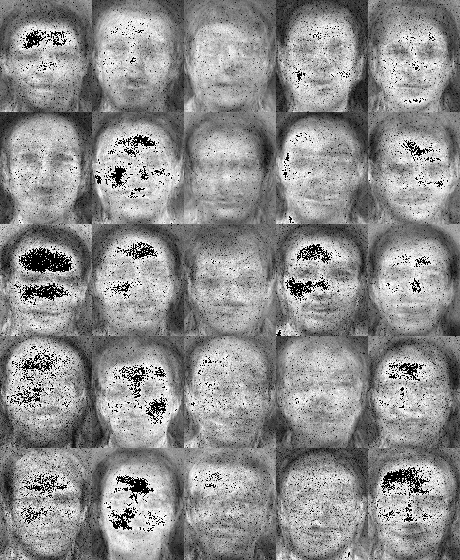
\includegraphics[width=.8\linewidth]{{betas=1/W_alph_0.1_alpw_1_beth_1_betw_1}.png}
		\caption{$\alpha_W = 1 $, $\alpha_H = 0.1 $}
	\end{subfigure}%
	\begin{subfigure}{.4\textwidth}
		\centering
		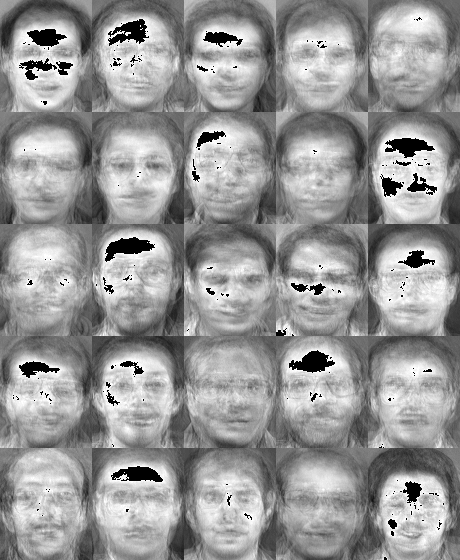
\includegraphics[width=.8\linewidth]{{betas=1/W_alph_0.1_alpw_10_beth_1_betw_1}.png}
		\caption{$\alpha_W = 10 $, $\alpha_H = 0.1$}
	\end{subfigure}%
	\caption{$W$ matrix for  $\beta_w = 1$ and $\beta_h = 1$, $\alpha_H = 0.1$}
\end{figure}   

\begin{figure}[H]
	\begin{subfigure}{.4\textwidth}
		\centering
		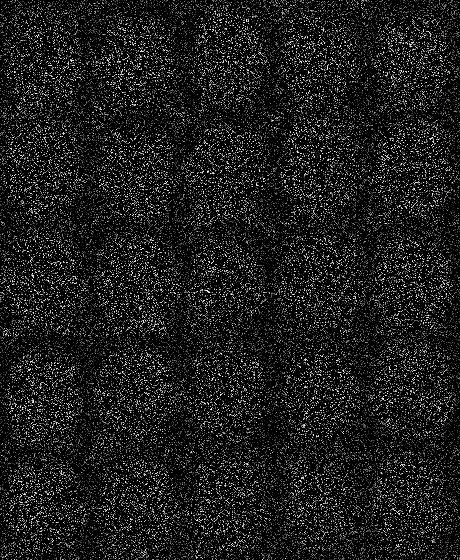
\includegraphics[width=.8\linewidth]{{betas=1/W_alph_0.5_alpw_0.1_beth_1_betw_1}.png}
		\caption{$\alpha_W = 0.1 $, $\alpha_H = 0.5 $}
	\end{subfigure}%
	\begin{subfigure}{.4\textwidth}
		\centering
		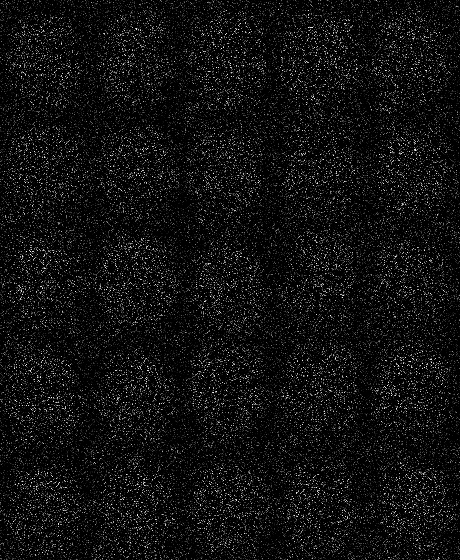
\includegraphics[width=.8\linewidth]{{betas=1/W_alph_1_alpw_0.1_beth_1_betw_1}.png}
		\caption{$\alpha_W = 0.1 $, $\alpha_H = 1$}
	\end{subfigure}%
	
	\begin{subfigure}{.4\textwidth}
		\centering
		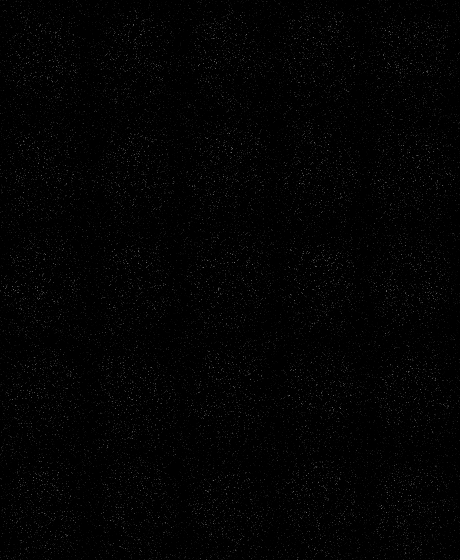
\includegraphics[width=.8\linewidth]{{betas=1/W_alph_5_alpw_0.1_beth_1_betw_1}.png}
		\caption{$\alpha_W = 0.1 $, $\alpha_H = 5 $}
	\end{subfigure}%
	\begin{subfigure}{.4\textwidth}
		\centering
		
\includegraphics[width=.8\linewidth]{{betas=1/W_alph_10_alpw_0.1_beth_1_betw_1}.png}
		\caption{$\alpha_W = 0.1 $, $\alpha_H = 10$}
	\end{subfigure}%

	\caption{$W$ matrix for  $\alpha_w = 1$ and $\alpha_h = 1$ and $\beta_W = 0.1 $}
\end{figure}   

\paragraph{Question 3}
The following figure shows the most relevant values of $\beta$, for $\alpha_w = 1$ and $\alpha_h = 1$

\begin{figure}[H]
	\begin{subfigure}{.4\textwidth}
		\centering
		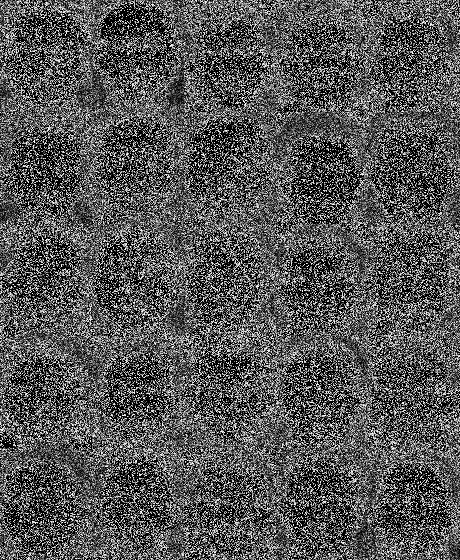
\includegraphics[width=.8\linewidth]{{alphas=1/W_alph_1_alpw_1_beth_0.1_betw_0.1}.png}
		\caption{$\beta_W = 0.1 $, $\beta_H = 0.1 $}
	\end{subfigure}%
	\begin{subfigure}{.4\textwidth}
		\centering
		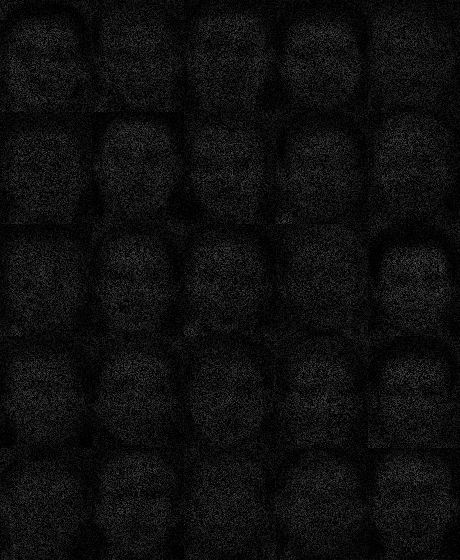
\includegraphics[width=.8\linewidth]{{alphas=1/W_alph_1_alpw_1_beth_0.1_betw_1}.png}
		\caption{$\beta_W = 1 $, $\beta_H = 0.1$}
	\end{subfigure}%
	
	\begin{subfigure}{.4\textwidth}
		\centering
		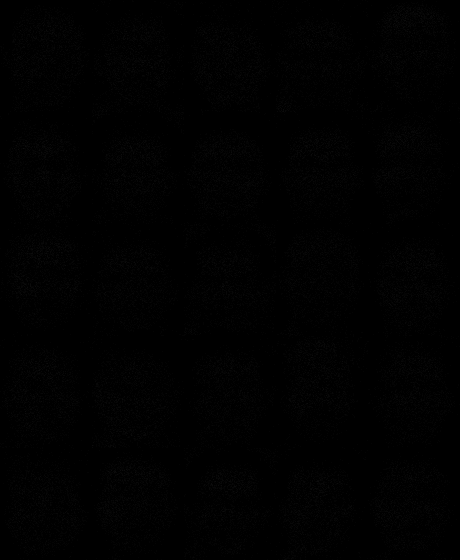
\includegraphics[width=.8\linewidth]{{alphas=1/W_alph_1_alpw_1_beth_0.1_betw_5}.png}
		\caption{$\beta_W = 5 $, $\beta_H = 0.1 $}
	\end{subfigure}%
	\begin{subfigure}{.4\textwidth}
		\centering
		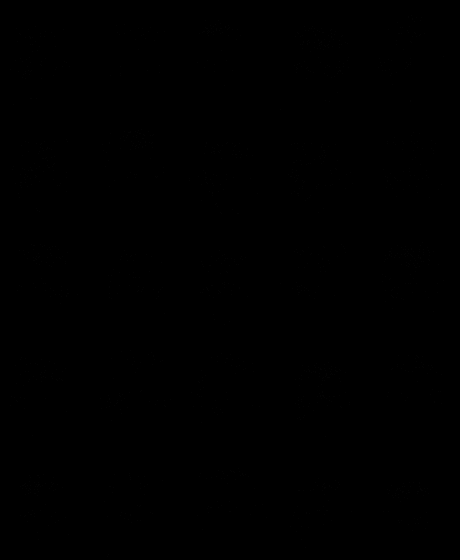
\includegraphics[width=.8\linewidth]{{alphas=1/W_alph_1_alpw_1_beth_0.1_betw_10}.png}
		\caption{$\beta_W = 10 $, $\beta_H = 0.1$}
	\end{subfigure}%

	\caption{$W$ matrix for  $\alpha_w = 1$ and $\alpha_h = 1$ and $\beta_H = 0.1 $}
\end{figure}   

\begin{figure}[H]
	\begin{subfigure}{.4\textwidth}
		\centering
		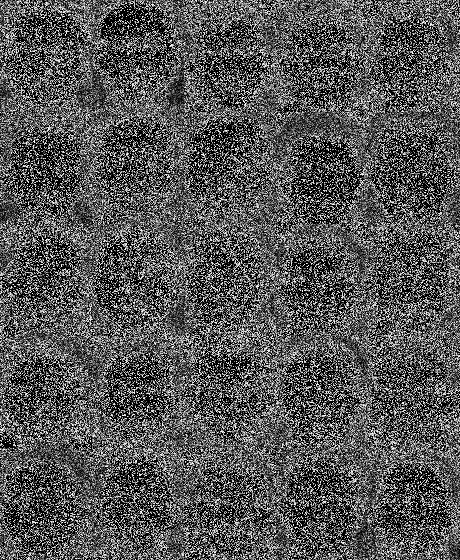
\includegraphics[width=.8\linewidth]{{alphas=1/W_alph_1_alpw_1_beth_0.1_betw_0.1}.png}
		\caption{$\beta_H = 0.1 $}
	\end{subfigure}%
	\begin{subfigure}{.4\textwidth}
		\centering
		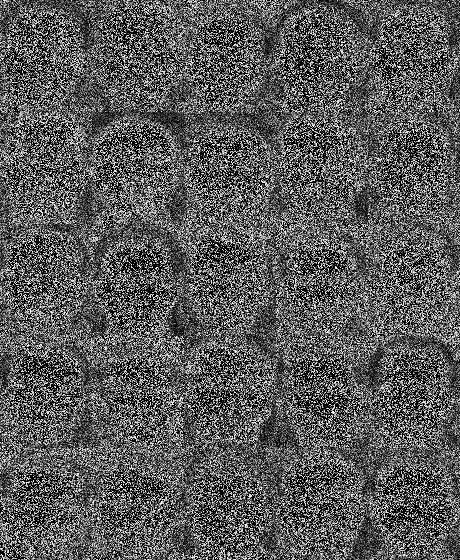
\includegraphics[width=.8\linewidth]{{alphas=1/W_alph_1_alpw_1_beth_1_betw_0.1}.png}
		\caption{$\beta_H = 1$}
	\end{subfigure}%
	
	\begin{subfigure}{.4\textwidth}
		\centering
		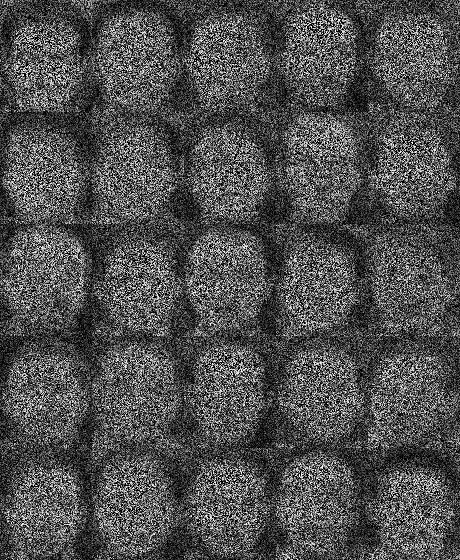
\includegraphics[width=.8\linewidth]{{alphas=1/W_alph_1_alpw_1_beth_5_betw_0.1}.png}
		\caption{$\beta_H = 5 $}
	\end{subfigure}%
	\begin{subfigure}{.4\textwidth}
		\centering
		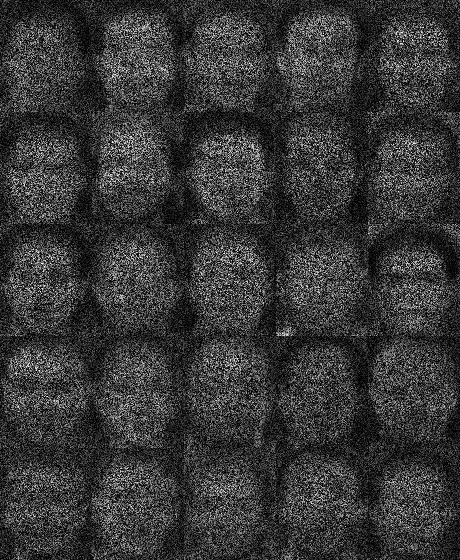
\includegraphics[width=.8\linewidth]{{alphas=1/W_alph_1_alpw_1_beth_10_betw_0.1}.png}
		\caption{$\beta_H = 10$}
	\end{subfigure}%

	\caption{$W$ matrix for  $\alpha_w = 1$ and $\alpha_h = 1$ and $\beta_W = 0.1 $}
\end{figure}   


\end{document}
